現在のホームページは大量の動的なコンテンツを含みユーザのエクスペリエンスを高めています。以前に比べてとても複雑になっています。いわゆる動的なコンテンツとはユーザの環境と要求に応じてWebアプリケーションが目的の内容を出力できることを指します。動的なホームページは"クロスサイトスクリプティング"(Cross Site Scripting、セキュリティ専門家が一般的にXSSと省略するもの)と呼ばれる攻撃を受けることがあります。

攻撃者は通常セキュリティホールのあるプログラム中にJavaScript、VBScript、ActiveXまたはFlashを挿入することでユーザを騙します。一旦攻撃が成功するとユーザアカウント情報が盗まれ、ユーザの設定を改ざんされてしまったり、cookieを盗みまたは汚染して悪意ある広告を埋め込んだりされます。

XSSに対する最も効果的な予防は以下の二種類を組み合わせることです:すべての入力データを検証し攻撃の検査をすること(これに関しては前の節でいくつかご紹介しました)。もうひとつは出力されるデータに対し適切な処理を行うことによってすでに挿入されてしまったいかなるスクリプトに対してもブラウザで実行されないようにすることです。

Goではどのようにこの効果的な防御を行なっているのでしょうか?Goのhtml/templateの中では以下のいくつかの関数によってエスケープすることができます。


\begin{itemize}
  \item func HTMLEscape(w io.Writer, b []byte) //bに対してエスケープを行い、wに出力する。
  \item func HTMLEscapeString(s string) string //sに対してエスケープを行い、結果の文字列を返す。
  \item func HTMLEscaper(args ...interface{}) string //複数の引数を同時にエスケープします。結果となる文字列を返します。
\end{itemize}

4.1節の例を見てみましょう。

\begin{lstlisting}[numbers=none]
fmt.Println("username:", template.HTMLEscapeString(r.Form.Get("username")))
//サーバ側に出力されます。
fmt.Println("password:", template.HTMLEscapeString(r.Form.Get("password")))
template.HTMLEscape(w, []byte(r.Form.Get("username")))
//クライアントに出力されます。
\end{lstlisting}

もし入力されたusernameが\texttt{<script>alert()</script>}だった場合、ブラウザ上では以下のように表示されます:

\begin{figure}[H]
  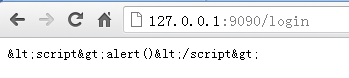
\includegraphics[width=8cm]{4.3.escape.png}
   \label{図4.3}
   \caption{Javascriptフィルターによる出力}
\end{figure}

Goのhtml/templateパッケージはデフォルトでhtmlタグをフィルターします。しかし時にはこの\texttt{<script>alert()</script>}を正常な情報として出力したい場合があるかもしれません。そのような場合はどのように処理するべきでしょうか?この場合はtext/templateをご利用ください。下の例をご覧ください: \texttt{import "text/template" ... t, err := template.New("foo").Parse(\{\{define "T"\}\}Hello, \{\{.\}\}!\{\{end\}\}) err = t.ExecuteTemplate(out, "T", "")}

出力

\begin{lstlisting}[numbers=none]
Hello, <script>alert('you have been pwned')</script>!
\end{lstlisting}

またはtemplate.HTML型を使用すると

\begin{lstlisting}[numbers=none]
import "html/template"
...
t, err := template.New("foo").Parse(`{{define "T"}}Hello,
                                    {{.}}!{{end}}`)
err = t.ExecuteTemplate(out, "T",
 template.HTML("<script>alert('you have been pwned')</script>"))
\end{lstlisting}

出力

\begin{lstlisting}[numbers=none]
Hello, <script>alert('you have been pwned')</script>!
\end{lstlisting}

\texttt{template.HTML}に変換した後も変数の内容はエスケープされません。

エスケープの例:

\begin{lstlisting}[numbers=none]
import "html/template"
...
t, err := template.New("foo").Parse(`{{define "T"}}Hello,
                                    {{.}}!{{end}}`)
err = t.ExecuteTemplate(out, "T",
           "<script>alert('you have been pwned')</script>")
\end{lstlisting}

エスケープ後の出力:

\begin{lstlisting}[numbers=none]
Hello, &lt;script&gt;alert(&#39;you have been pwned&#39;)&lt;/script&gt;!
\end{lstlisting}



